\documentclass{article}

\usepackage{graphicx}
\usepackage{authblk}
\usepackage{url}
\usepackage[german]{babel}
\usepackage{csquotes}
\usepackage{wrapfig}
\usepackage{biblatex}
\addbibresource{references.bib}

\graphicspath{ {./img/} }

\newcommand\blankpage{%
    \null
    \thispagestyle{empty}%
    \newpage}

\author[1]{Tobias Nöthlich}
\author[1]{Florian Richter}
\author[1]{Tim Krieg}

\title{Implementierung einer Testsuite zur Untersuchung von Möglichkeiten für DoS-Angriffe auf DTN-Protokollimplementierungen}





\begin{document}

\pagenumbering{arabic}


\begin{titlepage}

\begin{figure}[h]
\begin{flushleft}

\includegraphics[trim= 0 0 0 0 , clip, width=6cm]{img/logo.eps} 
\end{flushleft}
\end{figure}
\noindent
Fakultät Informatik\\
Institut für Systemarchitektur, Lehrstuhl Rechnernetze \\

\begin{center}
\Huge
\textbf{Implementierung einer Testsuite zur Untersuchung von Möglichkeiten für DoS-Angriffe auf DTN-Protokollimplementierungen} \\
\normalsize
\vspace{1cm}

\end{center}

\vspace{1cm}
\noindent
\textbf{\large{Tobias Nöthlich}} \\
\textbf{\large{Florian Richter}} \\
\textbf{\large{Tim Krieg}} \\

\vspace{1cm}
\noindent
{\LARGE Projektbericht} \\

\vspace{1cm}
\noindent
Betreuer\\
\textbf{\large{Dr.-Ing. Marius Feldman}} \\

\vspace{1cm}
\noindent
Wintesemester 2020/2021

\end{titlepage}
\tableofcontents

\newpage

\section{Einleitung}

\subsection{Motivation}
In Katastrophengebieten oder Verzögerungstolerante Netzwerke (engl. Delay-Tolerant Networking, kurz DTN)  
[PLATZHALTER] Generelles Intro über Nutzen von DTN in Raumfahrt, Katastrophenhilfe, etc \par
[PLATZHALTER] Kurz erklären wie das ganze funktioniert\par
[PLATZHALTER]Überleiten auf Angriffsvektoren $\rightarrow$ unsere Testsuite kommt ins Spiel.\par

\subsection{Anforderungen}

\begin{itemize}
\item Anforderungsanalyse
\end{itemize}

\section{Hintergrund und verwandte Arbeiten}

\subsection{DTN-Protokollimplementierungen}
[PLATZHALTER] Generelle \textbf{kurze} Einführung in die verschiedenen DTN-Implementierungen. 
\subsection{ION}
[PLATZHALTER] Kurze Erläuterung der ION DTN Implementation.
\subsection{CORE}
[PLATZHALTER] kurze Erläuterung zu CORE.\par

\section{Methodik}

\begin{itemize}
\item Erklärungen warum wir genau diese Frameworks gewählt haben
\item kurze Erläuterungen zu den Szenarien die wir uns ausgedacht haben
\end{itemize}

\section{Implementation}

\subsection{Shell Skripte}
\subsubsection{Setup}
\subsubsection{Start}
\subsubsection{...}
\subsection{Verknüpfung von ION und CORE}
\section{Szenarien}
\subsection{Bundle Flooding}
Das erste Szenario ist die Simulation eines Bundle Flooding Angriffs auf ein Netzwerkelement, das als Verbindungsstück zwischen einem Satelliten und dem Mission Control Center fungiert. Die für die Simulation genutzte Netzwerktopologie (siehe Abb. [PLATZHALTER]) besteht aus fünf Elementen, welche im Common Open Research Emulator durch den \textbf{Router} Knotentypen emuliert werden.\par
\begin{figure}[h]
\centering
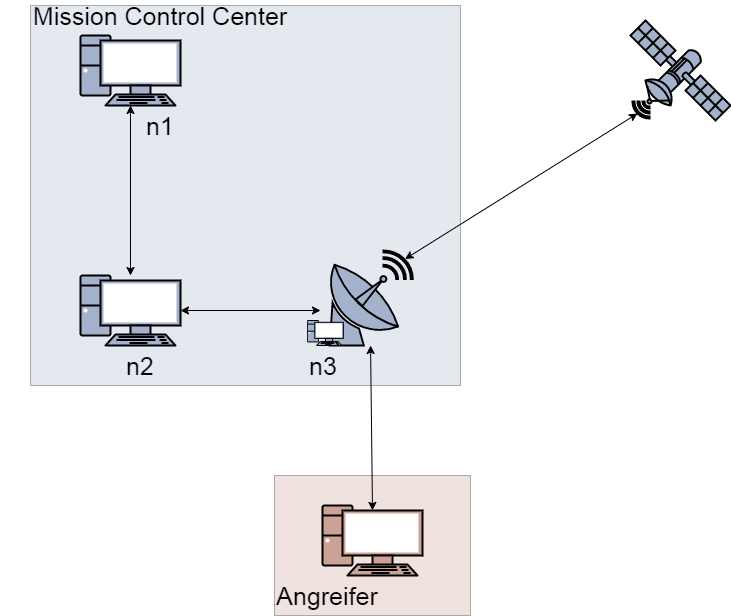
\includegraphics[width=0.5\textwidth]{flooding}
\caption{Netzwerktopologie des Bundle Flooding Szenarios}
\end{figure}
Das Grundprinzip des dem Szenario zugrunde liegenden Denial of Service Angriffs ist das Fluten des Zielsystems mit einer so großen Menge an Bundles, dass es nicht mehr in der Lage ist den legitimen Traffic zuzustellen. Da Delay-Tolerant Networking Systeme (DTN-Systeme) insbesondere für Gebiete, in denen stabile Verbindungen nicht durchgehend möglich sind, konzipiert wurden, gibt es auch in diesem Szenario Verbindungsunterbrechungen zwischen Satellit und dem Mission Control Center. Da durch unterbrochene Verbindungen nicht zustellbare Bundles zunächst auf dem letzten erreichbaren Knoten gesichert werden, muss ein Angreifer lediglich einen Knoten mit instabiler Verbindung attackieren. Es ist allerdings von Nöten, dass der Angreifer Zugriff auf ein in das ION-Netz eingebundenes System hat, da ION die verfügbaren Kontakte aus einer Konfigurationsdatei liest. Es ist also nicht möglich, von ausserhalb eine Verbindung zu einem bestehenden Netzwerk herzustellen.\par
Konkret auf unser Szenario bezogen bedeutet dies, dass der \textit{Angreifer} ein System im Netzwerk übernommen hat, und nun eine Verbindung zu \textit{n3} besteht. Er wird nun diesen Knoten mit an den \textit{Satelliten} adressierten Bundles fluten, bis  der restliche Netzwerkverkehr zum Erliegen kommt. Dabei reichen 50 Bundles pro Sekunde aus, um in kurzer Zeit die Übertragungskapazität der Leitung zwischen \textit{n3} und dem \textit{Satelliten} so zu verschlechtern, dass nur knapp ein Drittel der ursprünglichen Leistung für den restlichen Traffic zur Verfügung steht. Dies zeigt sich an den Round Trip Times (RTT) der Kommunikation zwischen \textit{n1} und dem \textit{Satelliten}. Hat ein Bundle Ping von \textit{n1} zum \textit{Satelliten} vor dem Start des DoS-Angriffs eine RTT von knapp einer Sekunde, so beträgt diese wenige Sekunden nach Start des DoS-Angriffs bereits über 3 Sekunden. Circa 5 Sekunden nachdem der \textit{Angreifer} beginnt \textit{n3} zu fluten, ist ein Ping von \textit{n1} zum \textit{Satelliten} nicht mehr möglich, da bereits über 100 Bundles vom \textit{Angreifer} auf dem Knoten \textit{n3} auf die Weiterleitung zum \textit{Satelliten} warten.\par
Ein wichtiger Faktor zum Erfolg dieses Angriffes, ist die von ION gegebene Möglichkeit, die Priorität der vom Bundle Ping ausgesendeten Bundles zu ändern. Durch das Versenden von Bundles mit der höchsten Priorität ist es dem \textit{Angreifer} möglich, die von ihm gesendeten Bundles an den Anfang der Queue zu setzen, die die Reihenfolge der weitergeleiteten Bundles festlegt. Des Weiteren sorgt die instabile Verbindung zwischen \textit{n3} und dem \textit{Satelliten}, welche alle 30 Sekunden für 30 Sekunden unterbrochen wird, für ein rapides Ansteigen der auf \textit{n3} zwischengelagerten Bundles. Die so von nicht legitimen Bundles circa 50 zu 1 dominierte Weiterleitungsqueue kann nicht mehr komplett geleert werden, was nach entsprechender Dauer zum Timeout der von \textit{n1} kommenden Bundles führt. \par
Zur Visualisierung der Attacke dienen zwei Shell-Skripte, welche  die Anzahl der auf jedem Knoten eingelagerten Bundles zeigen, sowie ein Skript, das den Ping von \textit{n1} zum \textit{Satelliten} visualisiert. Dieses Skript nutzt dabei zur besseren Übersicht die von ION zu Verfügung gestellten watch characters. So wird für jedes versendete Bundle einmal das Zeichen 'a' ausgegeben. Erreicht das auf so ausgelöste Acknowledgement \textit{n1}, wird desweiteren die RTT angezeigt. Die zur Visualisierung benötigten Skripte werden automatisch mit Start des Szenarios ausgeführt.

\subsection{DDoS Flooding}
Eine Weiterentwicklung des ersten Szenarios ist die Simulation eines Bundle Flooding Angriffs auf ein Netzwerkelement, das als Verbindungsstück zwischen einem Satelliten und dem Mission Control Center fungiert. Die für die Simulation genutzte Netzwerktopologie (siehe Abb. [PLATZHALTER]) besteht aus fünf Elementen, welche im Common Open Research Emulator durch den \textbf{Router} Knotentypen emuliert werden.\par
\begin{figure}[h]
\centering
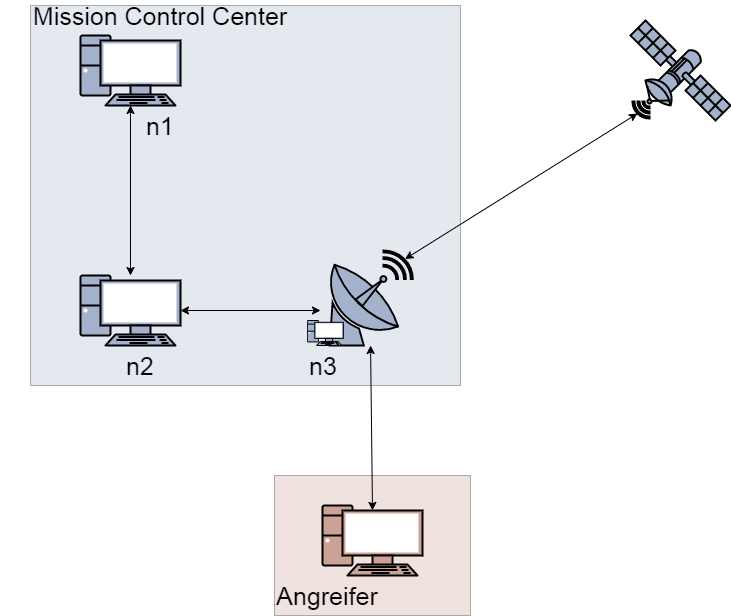
\includegraphics[width=0.5\textwidth]{flooding}
\caption{Netzwerktopologie des Bundle Flooding Szenarios}
\end{figure}

\subsection{Slowloris}
Im Gegensatz zu den bisher diskutierten Szenarios benötigen Application Layer Denial of Service Angriffe kein bereits kompromittiertes System um zu funktionieren. Das in diesem Abschnitt näher betrachtete Szenario setzt dabei einen Slowloris Angriff erfolgreich um. Wir nutzen in dem Szenario slowloris.py (Version 0.2.2; Yaltirakli, G., 2015)\cite{gkbrkslowloris}, ein Python Skript, welches die Attacke auf das Zielsystem ausführt.\par
Die hier simulierte Situation ist ein Angriff auf ein Katastrophenfrühwarnsystem. Die Netzwerktopologie (siehe Abb. [Platzhalter]) ist die Folgende:
\begin{itemize}
\item eine Messstation
\item ein Satellit für die Datenübermittlung
\item ein Kontrollzentrum
\item ein Emergency Broadcast System
\item ein Angreifer, der die Verbindung zwischen Messstation und Satellit stört
\end{itemize}
Dabei sind die Systeme des Frühwarnsystems in Reihe geschaltet und zusätzlich der Angreifer mit dem Satelliten verbunden. Als Transportprotokoll kommt TCP zum Einsatz.
Wie auch in den vorherigen Szenarien werden die einzelnen Knoten durch CORE Routerknoten emuliert.\par
\begin{figure}[h]
\centering
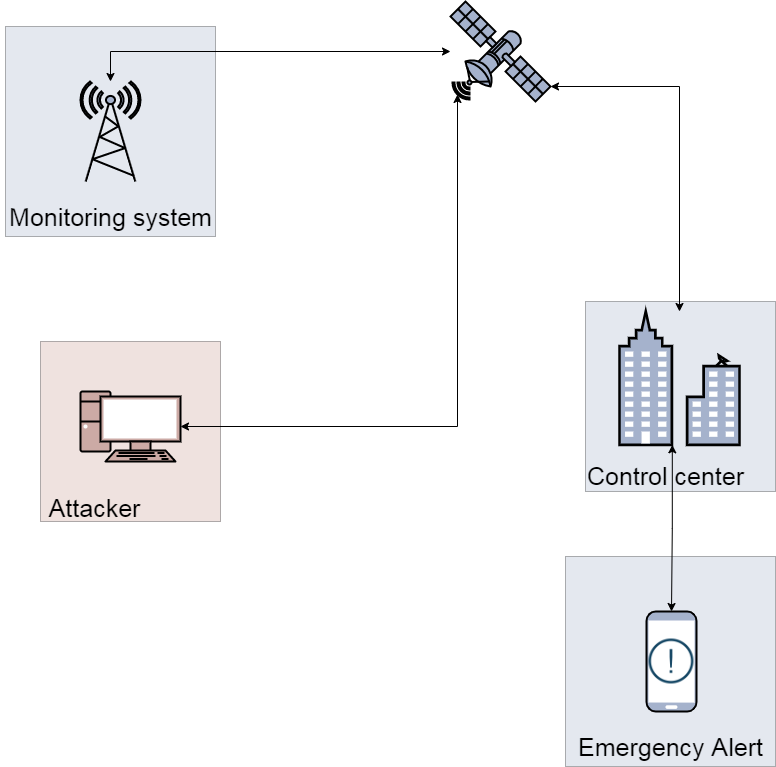
\includegraphics[width=0.5\textwidth]{slowloris}
\caption{Netzwerktopologie des Slowloris Szenarios}
\end{figure}
Das Ziel des Denial of Service Angriffs ist das Lahmlegen des Zielsystems unter minimaler Verwendung von Netzwerkressourcen. Dies wird erreicht, indem das Angreifersystem möglichst viele Verbindungen zum Zielsystem aufbaut und diese so lange wie möglich offenhält.\par
In diesem Szenario wird dieser Effekt durch das Ausführen von dem slowloris.py Skript auf dem Knoten, der den Angreifer simuliert, erreicht. Das Skript baut so viele Verbindungen wie möglich zu dem Satelliten auf und versendet nur Teilanfragen. Dies hat den Effekt, das auf dem Satelliten die Anfragen nie vollständig abgeschlossen werden, und die Verbindungen zum Angreifer bestehen bleiben. Werden auf diese Weise genügend Verbindungen gleichzeitig blockiert, so kann der Satellit von der  Messstation eingehende Verbindungsanfragen nicht annehmen und die Verbindung zwischen Messstation und Kontrollzentrum ist unterbrochen. Die Verbindungsunterbrechung tritt bereits den Bruchteil einer Sekunde nachdem der Angriff gestartet wurde auf und ist somit deutlich schneller als bei dem Bundle Flooding Angriff.\par
Diese Art Denial of Service Attacke zeichnet sich besonders dadurch aus, dass sie vollkommen vom ION-Netzwerk unabhängig ist, also kein bereits kompromittiertes System innerhalb des Netzwerkes benötigt wird, um erfolgreich die Verbindung zu stören. Ein Angreifer mit ausreichend leistungsstarker Hardware könnte damit sehr einfach sämtlichen Traffic in kritischen Systemen zum Erliegen bringen, sofern diese TCP als Tansportprotokoll nutzen.\par
Die Visualisierung der Auswirkungen des Angriffes in unserer Netzwerksimulation erfolgt wieder durch ein Shell-Skript, welches das Ergebnis des Pings von Messstation zum Kontrollzentrum in einer Konsole ausgibt. 

\section{Fazit und Ausblick}

\begin{itemize}
\item kurze Zusammenfassung
\item welche Anforderungen wurden erfüllt?
\item was könnte verbessert werden?
\item warum konnten verschiedene Anforderungen nicht erfüllt werden (hoffentlich nicht benötigt)
\end{itemize}



\newpage
\printbibliography
\end{document}
